\section{MicroNet}

MicroNet is a framework to develop and operate \ms{} applications. It is
designed to be especially support rich \ogs{}. MicroNet also provides all
needed to develop and operate an \og{}.

\subsection{Architecture Overview}

The deign concepts that build the foundation of MicroNet are derived from both
\ms{} and \og{} requirements. This leads to a set of concepts which is a union
of both \ms{} and \og{} principles.

\subsection{Dependency Abstraction}

\subsection{Networking}
Networking in MicroNet has been discussed in detail in project thesis one. This
section only provides a short summary of the topic.\\

Networking is the most fundamental aspect of an \og{} development and crucial
for the stability of \ms{} applications. The networking concept for \ms{}
applications is heavily influenced by the IDEAL tenet because it makes it
necessary to provide an abstract messaging concept that is decoupled from any
implementation.

In MicroNet this network abstraction is realized by defining a set of networking
capabilities that must be supported by the underlying network technology. These
capabilities are represented in the form of a Java interface. Standard services
can therefore communicate over the messaging interface injected by the
framework. This makes the underlying technology exchangeable. This allows
platform independence as long as the services are written in Java.

According to the polyglot programming tenet it is a requirement that arbitrary
technologies can participate in a \ms{} application. In this case an adapter
must be used to couple the external service with the application. The adapter
can be an be a implementation of the messaging interface in another language. In
this case the underlying messaging technology must provide an API for the
respective language. In the case of MicroNet ActiveMQ is used as the
message broker which provides a JMS API. JMS ports are also available for other
languages like for example the NMS API for C\#. This API is used to make the
Unity3D engine accessible from MicroNet.

To abstract underlying technical details it is assumed that all message
transfers of MicroNet are reliable (TCP). This is for the purpose of simplicity
over performance. Faster message transfers can be seen as an optimization but
this is not the topic of this thesis.

\subsubsection{Messaging System}

Messaging in MicroNet evolves around patterns: API Gateway, Reverse Proxy and
Pipes and Filters.\\

MicroNet uses a reverse proxy to interchange messages from the public Internet
with the internal network used by MicroNet. For this purpose two separate
message brokers are used and only the public broker is exposed to the Internet.
The gateway intercepts all messages from the public network and forwards them to
the responsible \ms{}. Messages are filtered by the

The reverse proxy is in fact also the API gateway. An API gateway is a standard
approach to offer the service API to the users. Upon reception of a message the
gateway can filter it according to a white- or blacklisting approach.

\subsubsection{User Sessions}

One challenge is to authenticate user connections. Since multiple gateways are
active simultaneously the user sessions are stored in the session store in
Couchbase. For unauthenticated connections the gateway only forwards login
messages to the login service. upon success the processing gateway adds the user
connection to the session store. Other gateways are then able to look up if a
connection is authenticated. The advantage of this solution is that it scales
very well. The downside is that it involves many reads to the session store.

A requirement for this approach to work is that the underlying networking
provides a way to correlate incoming messages with a connection. This can be
done generating a connection id hash based upon the user's IP/port combination.
ActiveMQ has this capability already built in by providing a globally unique
connection ID per connection.

\subsubsection{Messaging API}

This messaging API of MicroNet offers the following functionality to promote
stateless message transfers:

\begin{itemize}
  \item Sending a requests to a \ms{} either from a user or another \ms{}
  \item Sending a requests to a \ms{} and waiting for a response with a
  short\footnote{15 seconds seem appropriate for most short requests.} timeout
  either from a user or another \ms{}
  \item Sending an event to a user from a \ms{}
  \item Sending an event to a group of users from a \ms{}
  \item Sending a message to a topic, meaning to all subscribed \mss{}
  \item Named message parameters
\end{itemize}

These messaging capabilities are enough to model any arbitrary message transfer.
It leaves a great degree of freedom and makes message transfer implementation
very comfortable. 

\subsection{Consistency}

Consistency is a big concern in any distributed application and \ogs{} are no
exception. Although it is possible to categorize the consistency requirements
for games into strong consistency for sensitive data like account or payment
information and best effort consistency for all other game data. This aspect has
been highlighted in project thesis two \todo{cite thesis 2}.

The final solution to consistency in MicroNet is a solution to emphasis
exactly this two requirements. For strong consistency it is aways necessary that
one single service can process a complete transaction. This service then can
make a transaction ACID by using the two phase commit protocol offered by the
database. MicroNet uses ProstgreSQL for this purpose.

\subsection{Shared Model}

The general design of \mn{} is reclined to the design of modern game engines
like Unity3D or UnrealEngine 4. What these engines have in common is a graph to
describe the game e.g. all objects, levels, players, etc. which are part of the
game. This concept of game data organization will be referred as the game graph.
Two examples of game graphs are shown in \autoref{fig:scenegraph}. The game
graph as a logical concept 


\begin{figure}
  \centering
  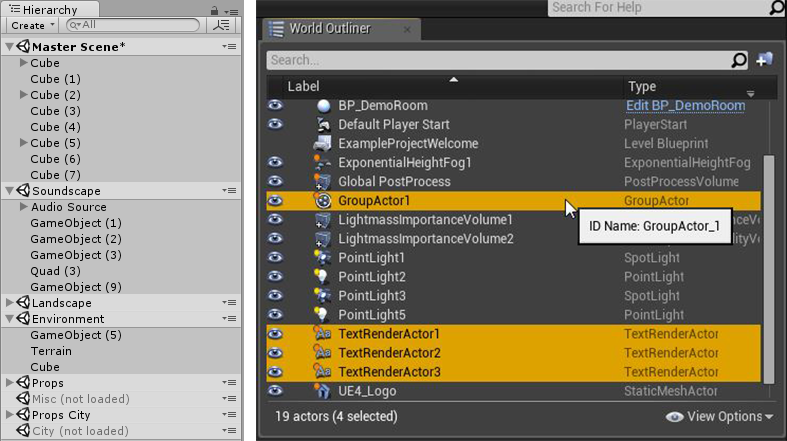
\includegraphics[width=\textwidth]{images/game_engine/scenegraph}
  \caption{Two example game graphs of the Unity3D (left) and the UnrealEngine4
  (right).}
  \label{fig:scenegraph}
\end{figure}

\subsection{Persistence}

\subsection{Shared API}

\subsection{Service Catalogue}







\subsection{MicroNet Tools}

\subsubsection{Annotations}
 (Design by contract)
 

\subsubsection{Code Generation}

\subsubsection{Code Assist}

\subsubsection{Service Explorer}

\paragraph{Build Configuration}

\paragraph{Run/Debug Configuration}

\subsubsection{Model Editor}

\subsubsection{Deployment}
















\subsection{OLD: Description of the MicroNet Framework}

Microservices reduce the complexity of an online game by splitting the game
domain into small shards that can be developed independently. These shards are
established by a domain driven design (DDD) approach. Each type of Microservice
is repsonsible to handle all aspects of the domain shard completly (cohesion).
This reduces the need to invest effort in inter service.\\

How does MicroNet help the developer to develop large online games:
\begin{itemize}
  \item MicroNet does not reinvent the wheel for online game development
  \item MicroNet works in conjunction with existing technologies, specifically popular game engines
  \item MicroNet tries to make the developer aware of the problems that are encountered during the development process
  \item While using MicroNet the developer learns the process of online game development 
  \item It helps the developers to get the difficult tasks like consistency of a
  asynchronous system right
\end{itemize}

What does MicroNet provide in this regard:
\begin{itemize}
  \item Provides a clear architecture for the game back-end
  \item Allows to develop individual game features independently
  \item Provides a simple protocol definition that helps the developers to loosely couple game features
  \item Offers standard solutions for technical requirements: Messaging
  functionality and Persistence functionality	
\end{itemize}

\subsection{Eclipse Tools}

Since MicroNet makes usage of various thirs party libraries and tools there
needs to be a way to manage them all. This purpose solves the Eclipse tools for
MicroNet. The MicroNet Tools is a set of plug-ins that are partially independent
of each other. They all help the developer to implement game specific \mss{}.

Since the UI of an Eclipse plug-in is written with the SWT library it can easily
be exported to a standalone tool that does not require Eclipse. However any code
related feature do require the Eclipse IDE.

\subsubsection{Service Generation}

Allows the developer to not worry about boiler plate code of setting up the
service in the framework. This covers the setup of the appropriate networking
solution according to the environment. This allows the developer to focus on the
actual service code.

\subsubsection{Code Assist}

The Code Assist plug-in helps the developer to keep track of functionality
provided by other services. It allows a type-safe communication between
services. The information that is needed to give these API proposals is
extracted from the service implementation at compile time. The information is
then shared via the version control system. This process is manually and the
developer must check in and probably merge his changes. 

The format of the distribute API description is not relevant because it is a
machine-readable format and the developer sees it in a polished form.

\subsubsection{Management UI}

The management UI plug-in helps the developer to get an overview over the whole
game application. It helps the manage the versions of services of the game
services as well as the versions of dependencies. This plug-in highly relies on
the description of the maven projects.

\subsection{PCG Solutions for Online Game}

\subsection{A Solution for \ms{} Development}